\chapter{Tìm hiểu 1}

% From IARJSET7
    Internet of Things (IoT) là mạng lưới các vật thể vật lý—thiết bị, dụng cụ, phương tiện, tòa nhà và các vật thể khác được nhúng với 
    thiết bị điện tử, mạch, phần mềm, cảm biến và khả năng kết nối mạng cho phép các vật thể này thu thập và trao đổi dữ liệu. Internet of Things 
    cho phép đọc dữ liệu đo đạc từ vật thể và điều khiển từ xa trên cơ sở hạ tầng mạng hiện có, tạo ra cơ hội tích hợp trực tiếp hơn thế 
    giới vật lý vào các hệ thống dựa trên máy tính nhằm cải thiện hiệu quả và độ chính xác.\par

    \section{Định nghĩa, khái niệm}
        Cơ sở hạ tầng mạng toàn cầu động với khả năng tự cấu hình 
        dựa trên các tiêu chuẩn và giao thức truyền thông. (Dynamic global network 
        infrastructure with self-configuring capabilities based on standards and communication protocols.)\par

        Vật thể vật lý và vật thể ảo trong IoT có định danh và thuộc tính riêng của chúng và có khả năng sử dụng giao diện thông minh và 
        được tích hợp như một mạng thông tin. Nói một cách dễ hiểu, IoT có thể được coi là một tập hợp các thiết bị được kết nối có 
        thể nhận dạng duy nhất. Các từ “Internet” và “Things” có nghĩa là một mạng lưới toàn cầu được kết nối với nhau dựa trên các 
        công nghệ cảm biến, truyền thông, mạng và xử lý thông tin, có thể là phiên bản mới của công nghệ thông tin và truyền thông 
        (ICT). Cho đến nay, một số công nghệ có liên quan đến IoT, chẳng hạn như mạng cảm biến không dây (WSN), mã vạch, cảm biến 
        thông minh, RFID, NFC, truyền thông không dây năng lượng thấp, điện toán đám mây, v.v.
 
    \section{Vị trí và vai trò}
    
    \section{Cấu trúc và nguyên lý}
        \subsection{Kiến trúc IoT}
            \subsubsection{SERVICE ORIENTED ARCHITECTURE}
                \paragraph{SENSING LAYER}
                    Sensing Layer được tích hợp với tất cả các đối tượng (vật thể) có sặn để thu thập dữ liệu trạng thái của chúng.
                \paragraph{NETWORK LAYER}
                    Network Layer là cơ sở hạ tầng hỗ trợ kết nối không dây hoặc có dây giữa các thiết bị.
                \paragraph{SERVICE LAYER}
                    Service Layer có nhiệm vụ tạo và quản lý các dịch vụ mà người dùng hoặc ứng dụng yêu cầu.
                \paragraph{INTERFACE LAYER}
                    Interface Layer bao gồm các phương thức tương tác với người dùng hoặc ứng dụng.

    \section{Các công nghệ, giao thức, chuẩn giao tiếp}

    \section{Các thiết bị IoT khả cấu hình trên thị trường}

% From jdaip
\chapter{Tìm hiểu 2}
    \section{Định nghĩa, khái niệm}
        Internet of Things (IoT) là một khuôn khổ trong đó mọi thứ đều có sự biểu diễn và hiện diện trên 
        Internet. Cụ thể hơn, Internet of Things hướng đến mục tiêu cung cấp các ứng dụng và dịch vụ mới bắc 
        cầu giữa thế giới vật lý và thế giới ảo, trong đó giao tiếp Máy-với-Máy (M2M) đại diện cho giao tiếp 
        cơ sở cho phép tương tác giữa Vạn vật và các ứng dụng trên đám mây. Điều này được định nghĩa bởi 
        tạp chí truyền thông IEEE.\par

        "Things" trong IoT có thể là bất kỳ thiết bị nào có bất kỳ loại cảm biến nào được nhúng với khả năng 
        thu thập dữ liệu và truyền dữ liệu qua mạng mà không cần can thiệp thủ công. Công nghệ nhúng trong 
        vật thể giúp tương tác với các trạng thái bên trong và môi trường bên ngoài, từ đó hỗ trợ quá 
        trình ra quyết định.\par
 
    \section{Vị trí và vai trò}
    
    \section{Cấu trúc và nguyên lý}
        \subsection{Kiến trúc 3 lớp}
            Kiến trúc này bao gồm ba lớp. Đầu tiên là Perception Layer, là lớp vật lý. Nó có các cảm 
            biến để đo đạc và thu thập thông tin về môi trường. Nó đo một số thông số vật 
            lý hoặc xác định các đối tượng thông minh khác trong môi trường. Thứ hai là Network Layer, 
            chịu trách nhiệm kết nối với các vật thông minh khác, thiết bị mạng và máy chủ. Nó cũng 
            được đặc trưng bởi việc truyền và xử lý dữ liệu cảm biến. Thứ ba là
            Application Layer có trách nhiệm cung cấp các dịch vụ cụ thể cho ứng dụng
            cho người dùng. Nó định nghĩa các ứng dụng khác nhau mà IoT có thể được 
            triển khai.\par

            \begin{figure}[h]
                \centering
                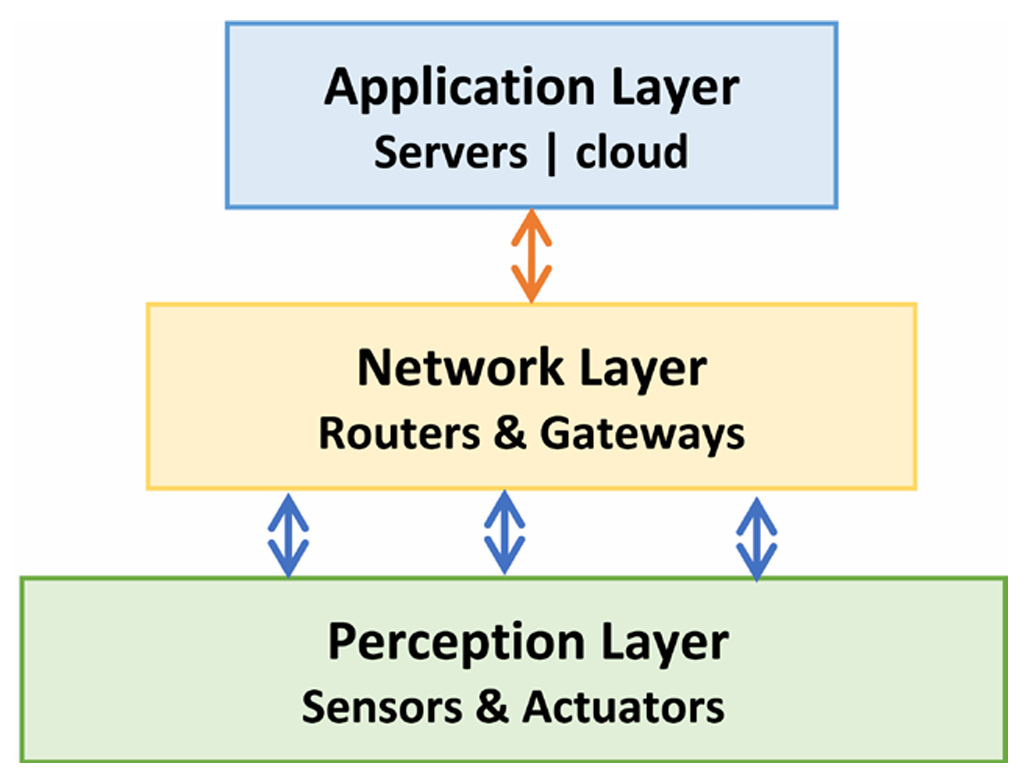
\includegraphics[width=0.8\textwidth]{figures/3_layer_architecture.png}
                \caption{Kiến trúc 3 lớp}
                \label{fig:3_layer_architecture}
            \end{figure}

        \subsection{Kiến trúc 5 lớp}
            Kiến trúc 5 lớp được thiết kế để xác định khái niệm hoàn chỉnh về chức năng và sự phát 
            triển của các thiết bị IoT. Cấu trúc mới bao gồm 5 lớp như thể hiện trong \autoref{fig:5_layer_architecture}.
            Perception Layer và Application Layer theo cùng cách như trong kiến trúc 3 lớp. Nhiệm vụ chính của
            Processing Layer là xử lý thông tin nhận được từ lớp mạng và đưa ra quyết định dựa trên kết quả đạt được 
            từ điện toán phổ biến.
            Transport Layer truyền dữ liệu cảm biến từ Perception Layer đến Processing Layer và ngược lại qua các mạng như
            mạng không dây, LAN, 3G, LTE, RFID và Bluetooth.
            Cuối cùng, Business Layer trực quan hóa thông tin và số liệu thống kê từ Application Layer và sử 
            dụng kiến thức này để lập kế hoạch cho các mục tiêu và chiến lược trong tương lai.\par

            \begin{figure}[h]
                \centering
                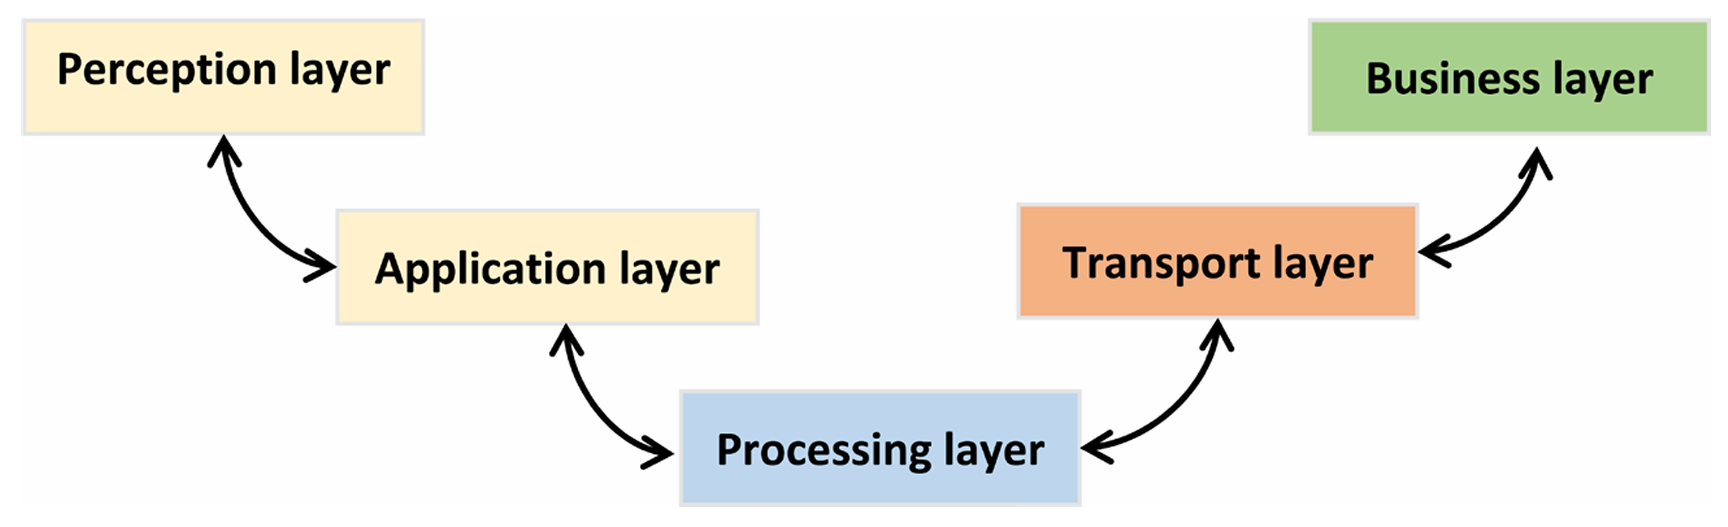
\includegraphics[width=0.8\textwidth]{figures/5_layer_architecture.png}
                \caption{Kiến trúc 5 lớp}
                \label{fig:5_layer_architecture}
            \end{figure}

    \section{Các công nghệ, giao thức, chuẩn giao tiếp}

    \section{Các thiết bị IoT khả cấu hình trên thị trường}

\chapter{Cái trên lộn rồi}
\chapter{Tìm hiểu IoT Gateway}
    \begin{figure}[h]
        \centering
        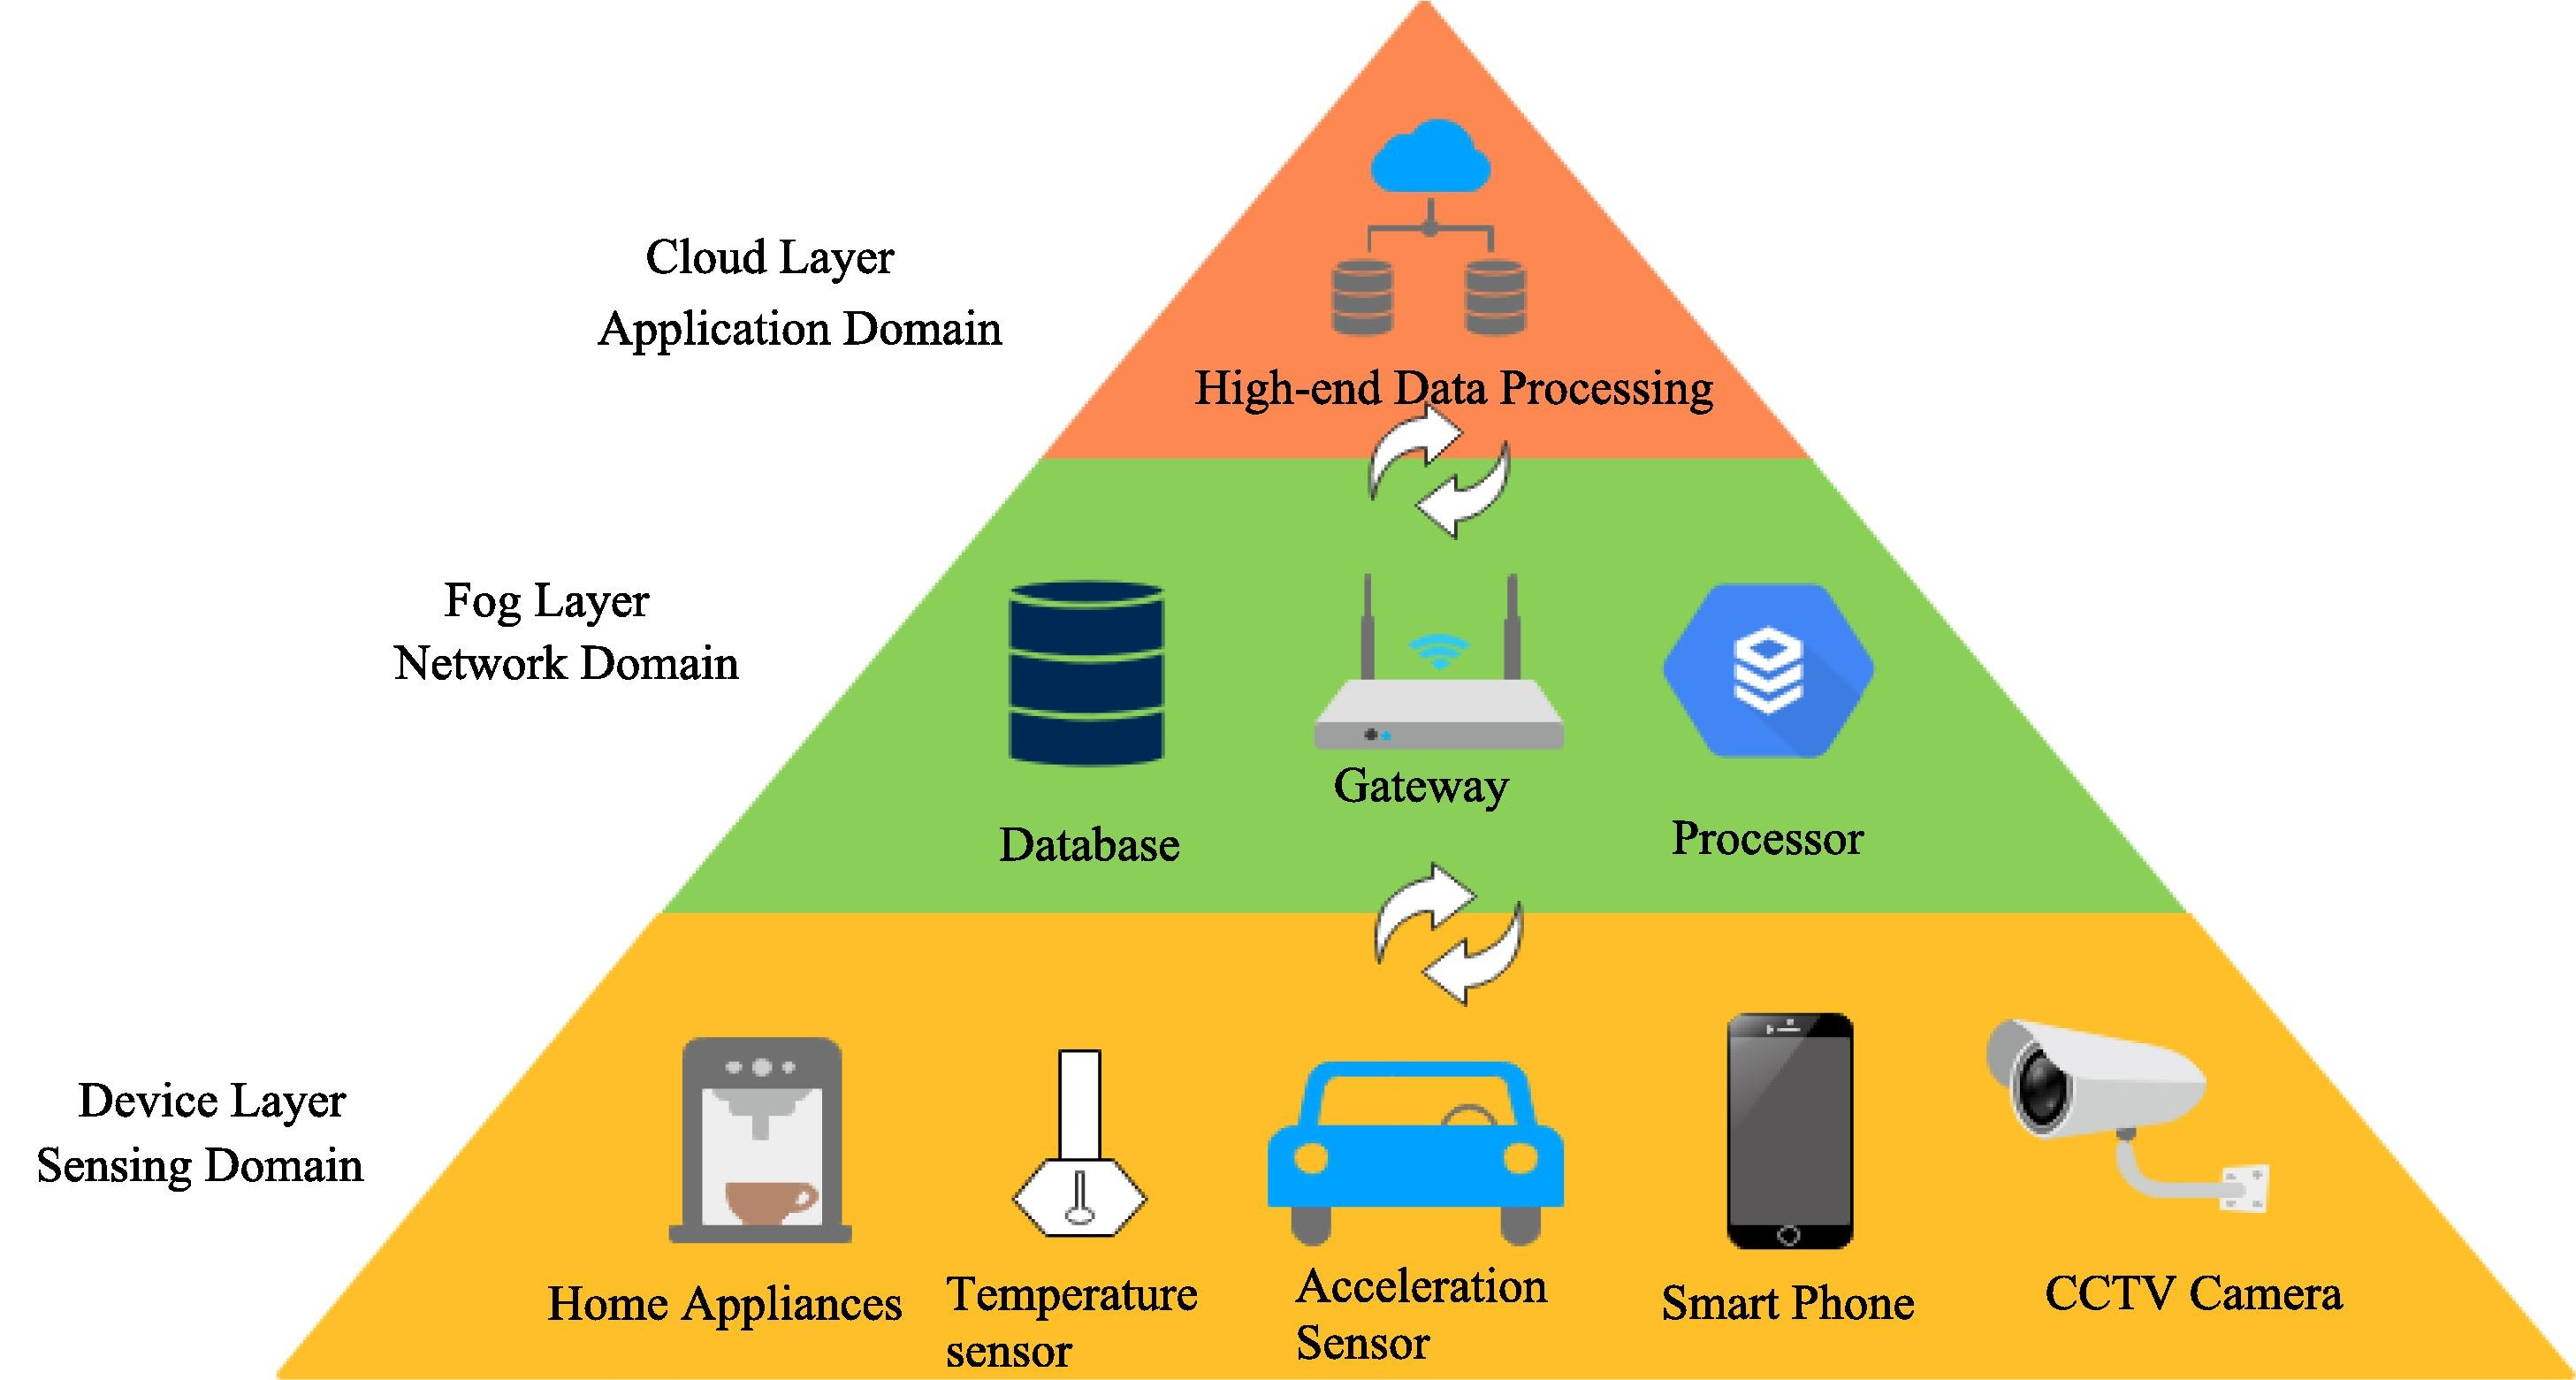
\includegraphics[width=0.8\textwidth]{figures/Gateway_in_IoT_architecture.jpg}
        \caption{Placement of Gateway in IoT architecture.}
    \end{figure}
    \section{Định nghĩa, khái niệm của IoT gateway}
        \textbf{Khái niệm:} Gateway trong lĩnh vực Internet of Things đóng vai trò là trung gian giữa nhiều 
        mạng cảm biến và nền tảng đám mây hoặc trung tâm dữ liệu được kết nối qua Internet. 
        
        

    \section{Vị trí và vai trò của IoT gateway trong hạ tầng IoT}
        Mục tiêu của nó là kiểm soát tính không đồng nhất do các thiết bị khác nhau tạo ra, 
        thu thập lượng lớn dữ liệu ở các định dạng khác nhau và chuyển tiếp dữ liệu đã thu 
        thập này lên một nền tảng cao hơn. Để hệ thống IoT hoạt động và quản lý đúng cách, dữ liệu thu 
        thập được phải được làm sạch, tiền xử lý và lọc trước khi gửi đến các trung tâm dữ 
        liệu dựa trên các ứng dụng cần thiết.
        Mục tiêu của nó là kiểm soát tính không đồng nhất do các thiết bị khác nhau tạo ra, 
        thu thập lượng lớn dữ liệu ở các định dạng khác nhau và chuyển tiếp dữ liệu đã thu 
        thập này lên một nền tảng cao hơn. Để hệ thống IoT hoạt động và quản lý đúng cách, dữ liệu thu 
        thập được phải được làm sạch, tiền xử lý và lọc trước khi gửi đến các trung tâm dữ 
        liệu dựa trên các ứng dụng cần thiết.
    \section{Cấu trúc và nguyên lý hoạt động cơ bản của các IoT gateway}
    \section{Các công nghệ, giao thức, và chuẩn giao tiếp được sử dụng phổ biến trong hạ tầng IoT}

    \section{Các thiết bị IoT gateway khả cấu hình đã có trên thị trường, tập trung vào các chức năng, đặc điểm nổi bật, công nghệ, giao thức, và các chuẩn giao tiếp được hỗ trợ}
